% Multiple Choice Question 17 to 18 (2 questions)

\textbf{See the instruction for questions \inteval{\value{question}+1} to \inteval{\value{question}+2}.} 

\begin{center}
    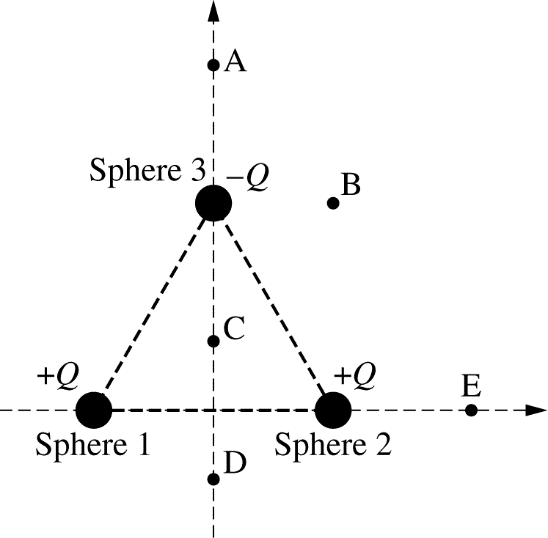
\includegraphics[scale=0.3]{images/img-010-018.png}
\end{center}

Three identical spheres are equally spaced from one another. Spheres 1 and 2 have charge $+Q$, and sphere 3 has a charge of $-Q$, as shown in the figure above. Five different positions are labeled A, B, C, D, and E. Positions A, B, and C are all the same distance from sphere 3. Positions C, D, and E are all the same distance from sphere 2. All spheres and points lie in the same plane.

% Multiple Choice Question 17
\begin{questions}
\setcounter{question}{16}
\question
The electric potential is highest at position

\begin{oneparchoices}
    \choice $A$
    \choice $B$
    \choice $C$
    \choice $D$
    \choice $E$
\end{oneparchoices}
\end{questions}

% Multiple Choice Question 18
\begin{questions}
\setcounter{question}{17}
\question
At which of the five positions are the horizontal and vertical components of the electric field directed toward the left and the top of the page, respectively?

\begin{oneparchoices}
    \choice A
    \choice B
    \choice C
    \choice D
    \choice E
\end{oneparchoices}
\end{questions}
